\section{Demazure weaves and braid varieties}\label{sec:weaves_braid_varieties}

Let $\beta\in\Br_n^+$ be a positive braid word in $n$-strands. In \Cref{sec:diagrammatic_weaves} we introduced the diagrammatic calculus of Demazure weaves $\w:\beta\to\delta(\beta)$, cf.~\Cref{ssec:summary_Demazure_weaves}. In this section we start to explore a use of such diagrammatic weave calculus: studying the geometry of a certain smooth affine variety $X(\beta)$ associated to $\beta$, known as its braid variety. Braid varieties include and generalize many interesting instances of varieties appearing in Lie theory and parts of algebraic geometry, see \Cref{ssec:braid_varieties_examples}. A central result on such braid varieties, which we approach and establish via Demazure weaves, is that their coordinate ring of regular functions admits the structure of a cluster algebra. The quiver and cluster variables of many cluster seeds for these cluster algebras can be described via the diagrammatic calculus of Demazure weaves.

\begin{comment}
\color{purple} {\bf TO BE EDITED}
\noindent The object of this section is to define braid varieties, provide examples and discuss some properties. The key definition is \cref{def:braid_variety} in \cref{ssec:braidvarieties_def}. Examples are provided in \cref{ssec:braid_varieties_examples}. Invariance properties, including independence of braid word and a torus action, are presented in \cref{ssec:braid_varieties_invariance}. See \cref{lem:braid_invariance} and \cref{lem:torusaction_coordinates}. A useful coordinate system to describe braid varieties is then introduced in \cref{ssec:braid_varieties_coordinates}, cf.~\cref{lem:equations_braidvar}.
\color{black}
\end{comment}
%%%%%%%%%%%%%%%%%%%%%%%%%%%%%%%%%%%%%%%%%%%%%
%%%%%%%%%%%%%%%%%%%%%%%%%%%%%%%%%%%%%%%%%%%%%

\subsection{Definition of braid varieties}\label{ssec:braidvarieties_def} Let $\G$ be a simple algebraic group with Weyl group $W(\G)$. We fix a Borel subgroup  $\borel\sse\G$, a Cartan subgroup $\T\subset \borel$ and consider the flag variety $\G/\borel$. As before, for the sake of the exposition, we focus on $\G=\SL_n$ and thus $W(\SL_n)\simeq S_n$ is the permutation group on $n$ elements. We can also fix $\borel$ to be the subgroup of special upper-triangular matrices and $\T$ the subgroup of special diagonal matrices. In this case, the flag variety $\SL_n/\borel$ has dimension $n(n-1)/2$.\\

Pairs of flags $\borel_1,\borel_2\in \G/\borel$ in relative position $w\in W(\G)$, i.e.~$\borel_1=[g_1\borel]$ and $\borel_2=[g_2\borel]$ such that $g_1^{-1}g_2\in \borel w\borel$, are denoted by $\borel_1 \buildrel w \over \longrightarrow \borel_2$. Braid varieties are defined as follows:\\

\begin{fdef}\label{def:braid_variety}
Let $\beta = \sigma_{i_1}\cdots \sigma_{i_{\ell}}$ be a positive braid word and $\delta(\beta) \in W(\G)$ its Demazure product. The {\it braid variety} associated with $\beta$ is
\begin{equation}\label{eq:braid_variety}
X(\beta) := \{(\borel_1, \dots, \borel_{\ell+1}) \in (\G/\borel)^{\ell + 1} \mid \borel_1 = \borel, \borel_{k} \buildrel s_{i_{k}} \over \longrightarrow \borel_{k+1}, \borel_{\ell + 1} = \delta(\beta) \borel \},
\end{equation}
\noindent where $\delta(\beta) \in W(\G) \cong N_{\G}(\T)/\T$ has been lifted to $N_{\G}(\T)$; this is well-defined since the flag $\delta(\beta) \borel$ does not depend on such a lift.
\end{fdef}
\vspace{0.2cm}
\noindent That is, \textcolor{blue}{$X(\beta)$ parametrizes linear configurations of flags whose consecutive relative positions are dictated by the word $\beta$ and their ends are fixed}: they start with the standard $\borel$ and end with $\delta(\beta)\borel$. A few comments on Definition \ref{def:braid_variety}:
\begin{itemize}
    \item[(i)] The flag variety $\G/\borel$ is a projective variety, and thus so is the Cartesian product $(\G/\borel)^{\ell + 1}$. By choosing appropriate coordinates, we can show that the subset $X(\beta)\sse (\G/\borel)^{\ell + 1}$ is itself an affine variety. It is smooth, irreducible, of dimension $\ell(\beta)-\ell(\delta(\beta))$ and defined over $\Z$, cf.~\Cref{lem:equations_braidvar}. Note that its dimension is independent of the rank of $\G$, e.g.~independent of the number $n$ of strands in $[\beta]\in\Br(\G)$ for $\G=\SL_n$.\\

    \item[(ii)] A braid word $\beta$ is used to define $X(\beta)$, but the isomorphism type of $X(\beta)$ as an affine variety only depends on the braid $[\beta]\in\Br(\G)$. In fact, we will explain that each braid move in $\Br(\G)$, from a braid word $\beta_1$ to another $\beta_2$, with $[\beta_1]=[\beta_2]$, gives an explicit isomorphism $X(\beta_1)\cong X(\beta_2)$. In addition, if two braid words $\beta_1,\beta_2$ differ by cyclic rotation $\s_i\beta\to\beta\s_{n-i}$ and $\delta(\beta_1)=w_0$, we still have an explicit isomorphism $X(\beta_1)\cong X(\beta_2)$, despite the braids $[\beta_1]\neq[\beta_2]$ being different. See \cref{ssec:braid_varieties_invariance} below for details.\\

    \item[(iii)] At this stage, $X(\beta)$ is defined only using the information of $\beta$. As we move forward, we study the geometry of $X(\beta)$ by using different Demazure weaves $\w:\beta\lr\delta(\beta)$. So, to emphasize, Demazure weaves are {\it not} used in the definition of $X(\beta)$.
\end{itemize}

\begin{center}
	\begin{figure}
		\centering
		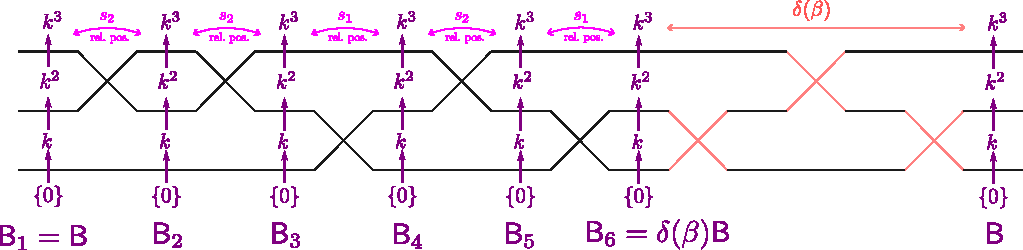
\includegraphics[width=\textwidth]{figures/BraidVarietyDef1.pdf}
		\caption{A visualization of the linear configuration of flags parametrized by $X(\beta)$, with $\beta=\sigma_2^2\s_1\s_2\s_1$. The crossings corresponding to $\delta(\beta)=w_0=\s_1\s_2\s_1$ are drawn in orange.}
		\label{fig:BraidVariefyDef1}
	\end{figure}
\end{center}

\begin{remark}\label{rmk:borels_flags} Since we focus on $\G=\SL_n$, we can switch between Borel subgroups of $\SL_n$ and full flags in $k^n$, understood as nested sequences
$$\{0\}\subset k\subset k^2\subset\ldots \subset k^n$$
of linear subspaces of $k^n$.\footnote{Technically this discussion also applies to $\Z$-modules and we use $\Z$ as the ground ring throughout. We focus here on a field $k$ and $k$-vector spaces for clarity, which we can do by base change.} The Borel subgroup that corresponds to a given full flag is given by all the elements $g\in\SL_n$ that leave that particular flag invariant. That is, given the flag $g\borel$, the stabilizer is the Borel subgroup of matrices of the form $g\borel g^{-1}$, i.e.~$\G$ acting by conjugation. For instance, given the standard basis $\{e_i\}$ of $k^n$, the Borel subgroup corresponding to the standard flag
$$\{0\}\subset \langle e_1\rangle\subset \langle e_1,e_2\rangle\subset\ldots \subset \langle e_1,e_2,\ldots,e_n\rangle,$$
is the subgroup $\borel\sse\SL_n$ of upper-triangular matrices. That corresponding to the antistandard flag
$$\{0\}\subset \langle e_n\rangle\subset \langle e_{n-1},e_n\rangle\subset\ldots \subset \langle e_1,e_2,\ldots,e_n\rangle,$$
is the opposite subgroup $\borel_-$ of lower-triangular matrices. In terms of matrices, this corresponds to the fact that $w_0Bw_0$ is a lower-triangular matrix if $B\in\borel$ is upper-triangular, where we used a permutation matrix to lift $w_0$ from $W(\G)$ to $\G$.
\begin{comment}
In terms of matrices, this corresponds to the fact that $w_0Bw_0$ is a lower-triangular matrix if $B\in\borel$ is upper-triangular, where we use the permutation matrix for $w_0$:
$$w_0=\left(\begin{matrix}
0 & 0 & \ldots & 0 & 1\\ 
0 & 0 &  \ldots & 1 & 0 \\
0 &  0 & \ldots & 0 &0 \\ 
\vdots & \vdots & \ddots & \vdots & \vdots \\
1 & 0 & \ldots & 0 & 0
\end{matrix}\right)\in \SL_n.$$
\end{comment}
Under the identification between Borel subgroups of $\SL_n$ and full flags in $k^n$, the $i$-dimensional subspace of the full flag associated to a Borel $\borel\sse\G$ is denoted by $\borel^i$. Then $\borel_1\stackrel{s_i}{\to}\borel_2$ if and only if the associated flags differ {\it exactly} at the $i$ dimensional subspace, i.e.~ $\borel_1^k=\borel_2^k$ if $k\neq i$ and $\borel_1^i\neq\borel_2^i$. The standard and antistandard flags above are in $w_0$-relative position, as transverse as possible: $\borel^j\cap(\borel_-)^{n-j}=\{0\}$ for all $j\in[0,n]$.\sbs
\end{remark}

In this $\G=\SL_n$ case, and with \Cref{rmk:borels_flags}  in mind, it can be helpful to visualize Definition \ref{def:braid_variety} as follows. First, draw horizontally the braid diagram for $\beta$ in the plane $\R^2$ and assign vector spaces in the open regions $\R^2\setminus\beta$ according to the following rule: the unbounded region below $\beta$ has $\{0\}$, the region above has $k^n$ and, in general, a bounded region is assigned the vector space $k^i$ if and only if it has $i$ strands of $\beta$ below it; cf.~Figure \ref{fig:BraidVariefyDef1}. Second, the tuple of flags $(\borel_1, \dots, \borel_{r+1})$ can then be thought of as drawing a vertical segment in between each pair of crossings of $\beta$ and choosing injective linear maps $k^i\lr\ k^{i+1}$ going upwards. This is drawn in Figure \ref{fig:BraidVariefyDef1} in an example, where the flags are emphasized in purple. Third, the two conditions cutting out $X(\beta)\sse (\G/\borel)^{\ell + 1}$ in Definition \ref{def:braid_variety} are of two types:

\begin{enumerate}
    \item {\it Transversality conditions}: for each crossing $\sigma_{i_k}$ of $\beta$, the flags at the left and right of the crossing are in $s_{i_k}$-relative position. That is, all subspaces of the flags at the left and right of the crossing coincide except the $i_k$-dimensional subspace, which is forced to be different, cf.~\cref{rmk:borels_flags}. This transversality condition is indicated in pink in Figure \ref{fig:BraidVariefyDef1}.\\

    \item {\it Boundary conditions}: the first flag is forced to be standard, so $\borel_1=\borel$, and the last one ``as antistandard as possible'', so $\borel_{r + 1} = \delta(\beta) \borel$. If $\delta(\beta)=w_0$, which is an important case, then it is literally the antistandard flag. From a visual viewpoint, these boundary conditions allow us to essentially think of the tuple as being cyclic, so the right part of $\beta$ connects back to its left part in Figure \ref{fig:BraidVariefyDef1}.
\end{enumerate}


\begin{example}\label{ex:permutation_vs_braid} $(1)$ Consider the case where $\beta=s$ is the lift of a permutation $s\in W(\G)$, i.e.~each pair of strands intersects at most once. \cite[Lemma 3.1]{CGGLSS25} shows that given two flags $\FF_1,\FF_2$ in relative position $\FF_1\stackrel{s}{\to}\FF_2$, then the $(\ell(s)-1)$ intermediate flags between $\FF_1$ and $\FF_2$ are uniquely determined by $\FF_1$ and $\FF_2$.\\

\noindent $(2)$ For a general braid word $\beta$, the fact in (1) is not true. Namely, for almost any braid diagram for a $\beta$, with two fixed flags $\FF_1,\FF_2$ left and right of this diagram, the space of intermediate flags between $\FF_1$ and $\FF_2$ is positive dimensional. In fact, $X(\beta)$ is zero-dimensional if and only if $\beta$ is a permutation braid. In this case where $\beta$ is a permutation, $X(\beta)$ is a point. This is a starting point for braid varieties: the transversality conditions for $X(\beta)$, which can be abbreviated $\borel\stackrel{\beta}{\to}\delta(\beta)\borel$, typically define a moduli of tuples of flags of non-zero dimension with rather rich geometry. For more details on relative position of flags, see e.g.~\cite[Section 3.2]{CGGLSS25}.\sbs
\end{example}

\begin{center}
	\begin{figure}
		\centering
		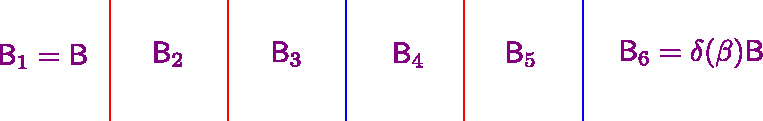
\includegraphics[scale=1]{figures/BraidVariety_DiagramExample.pdf}
		\caption{A visualization of the linear configuration of flags parametrized by $X(\beta)$, with $\beta=\sigma_2^2\s_1\s_2\s_1$, which is closer to the diagrammatics of weaves. Here a blue vertical line indicates a $\s_1$-label and a red vertical line indicates a $\s_2$-label. Since we label blue and red weave edges by $\s_1$ and $\s_2$ respectively, two flags which are to the left and right of a vertical blue strand must be in $s_1$-relative position, whereas two flags which are to the left and right of a vertical red strand must be in $s_2$-relative position.}
		\label{fig:BraidVariety_DiagramExample}
	\end{figure}
\end{center}
%\noindent \cref{ex:permutation_vs_braid} is a starting point for braid varieties: the transversality conditions for $X(\beta)$, which can be abbreviated $\borel\stackrel{\beta}{\to}w_0\borel$, typically define a moduli of tuples of flags of non-zero dimension with rather rich geometry. For more details on relative position of flags, see e.g.~\cite[Section 3.2]{CGGLSS25}.\\
\subsubsection{Braid varieties via weave diagrams}\label{sssec:first_connection_weave_diagrams} Given $\beta\in\mbox{Br}_n^+$, and to start connecting with the diagrammatic calculus of Demazure weaves in \Cref{sec:diagrammatic_weaves}, we can also represent points in the braid variety $X(\beta)$ as follows:

\begin{enumerate}
    \item As in \Cref{ssec:primer_Demazure_weaves}, we draw the positive braid word $\beta=\s_{i_1}\cdots \s_{i_\ell}\in \mbox{Br}_n^+$ as a set of $\ell$ parallel vertical strands on the plane, with the $j$th strand from the left labeled by $\s_{i_j}$.\\

    \item In each space in between two such parallel vertical strands we assign a flag in $\G/\borel$.\\

    \item In such a diagrammatic representation, the two flags $\borel_l,\borel_r$ respectively to the left and to the right of a vertical strand corresponding to $\s_{i_j}$ (labeled by $s_{i_j}$) are forced to be in $s_{i_j}$-relative position, i.e.~$\borel_l\stackrel{s_{i_j}}{\to}\borel_r$.\\

    \item The leftmost and rightmost flags are forced to be the standard flag $\borel$ and the $\delta(\beta)\borel$, respectively.
\end{enumerate}

\noindent For instance, \Cref{fig:BraidVariety_DiagramExample} illustrates the configuration of flags in \Cref{fig:BraidVariefyDef1} using these diagrammatic rules. This hints towards a first important relation between braid varieties and Demazure weaves: a Demazure weave $\w:\beta\to\delta(\beta)$ will allow us to study the braid variety $X(\beta)$, where $X(\beta)$ will appear by considering flags along the north boundary of $\w$, as in \Cref{fig:BraidVariety_DiagramExample}.\\

\noindent In general, given a Demazure weave $\w:\beta\to\delta(\beta)$, a horizontal slice $h$ away from a weave vertex determines a positive braid word $\beta_h$. In particular, we can assign the braid variety $X(\beta_h)$ to a horizontal slice $h$. For instance, the braid variety $X(\beta)$ corresponds to a horizontal slice at the north boundary of $\w$. The braid variety corresponding to the horizontal slice at the south boundary is $X(\delta(\beta))\cong\{\mbox{pt}\}$, which is a point by \cref{ex:permutation_vs_braid}.(2).

\begin{remark}
In this sense, if a Demazure weave $\w:\beta\to\delta(\beta)$ can be understood as a way of simplifying $\beta$ down to the permutation $\delta(\beta)$, via braid moves and $\s_i^2\to\s_i$ moves, then the same principle applies to the braid variety $X(\beta)$. Namely, a Demazure weave $\w:\beta\to\delta(\beta)$ provides a way to find smaller and smaller open subsets of $X(\beta)$, which we will see ultimately yield an open toric embedding $\iota_\w:(\bG_m)^d\lr X(\beta)$, with $d={\dim X(\beta)}$, see \Cref{cor:weave_to_toric_embedding} below.\sbs
\end{remark}

%%%%%%%%%%%%%%%%%%%%%%%%%%%%%%%%%%%%%%%%%%%%%
%%%%%%%%%%%%%%%%%%%%%%%%%%%%%%%%%%%%%%%%%%%%%
%%%%%%%%%%%%%%%%%%%%%%%%%%%%%%%%%%%%%%%%%%%%%

\subsection{Examples of braid varieties}\label{ssec:braid_varieties_examples} Certain varieties studied in the context of representation theory, algebraic geometry and algebraic combinatorics, are \color{blue}instances of braid varieties\color{black}:\\

{\bf 1.} The \color{blue}{\it open Richardson variety} \color{black} $\SR_{u,v}\sse \G/\B$ is defined as the intersection
        $$\SR_{u,v}:=(BvB/B)\cap (B_-uB/B)$$
        of the Schubert (and opposite Schubert) cells associated to two permutations $u,v\in W(\G)$ with $u\leq v$. Then, the open Richardson variety $\SR_{u,v}\sse \G/\B$ is isomorphic to the braid variety $X(\beta_{u,v})$, with
        $$\beta_{u,v}=\beta(v)\beta(u^{-1}w_0),\quad u,v\in W(\G),$$
        where $\beta(s)$ denotes the braid lift of a reduced permutation $s\in W(\G)$ to the positive braid monoid, and $w_0\in W(\G)$ is the longest element, a.k.a.~the half-twist. This is proven in \cite[Section 4]{CGGS2} and \cite[Section 3.6]{CGGLSS25}.\\

{\bf 2.} The \color{blue}{\it open positroid varieties} \color{black} $\Pi_{u,v}\sse\Gr(k,n)$ are smooth subvarieties of the Grassmannian $\Gr(k,n)$, indexed by two permutations $u,v\in W(\G)$ with $v$ satisfying a certain combinatorial property (being $k$-Grassmannian). Following the Richardson case $(1)$ above, each positroid $\Pi_{u,v}\sse\Gr(k,n)$  is isomorphic to the braid variety $X(\beta_{u,v})$, with
        $$\beta_{u,v}=\beta(v)\beta(u^{-1}w_0),\quad u,v\in W(\G).$$
        This is proven in \cite[Theorem 1.3]{CGGS2}. For instance, the braid variety for the top-dimensional (open) positroid $\Pi_{u,v}\sse\Gr(k,n)$ is given by the braid (typically) associated to the $(k,n+k)$-torus link.\\
        
        The relation between open positroid varieties and open Richardson varieties is explained in \cite{KLS,KLS2}; see also the survey \cite{speyer2024richardsonvarietiesprojectedrichardson}. At its core, the former are projections of the latter, under the natural projection from the (complete) flag variety $\G/\borel$ to the Grassmannian $\Gr(k,n)$, seen as a partial flag variety. Notably, unlike a general Richardson variety, positroid varieties are also described by many other combinatorial gadgets, different from the pair $(u,v)$. These include $k$-bounded affine permutations $f$, cyclic rank matrices $r$, and Le diagrams $\Le$. It is explained in \cite{CGGS2} how to extract braids $J_k(f),M_k(r),D_{k}(\Le)$ associated to each of these combinatorial objects so that the associated braid varieties are isomorphic to the given positroid variety.\\

{\bf 3.} As precursors of $(1)$ and $(2)$ above, \color{blue}{\it double Bruhat cells} \color{black} were one of the first classes of varieties to be studied cluster-theoretically, cf.~\cite{FZ1999}. The double Bruhat cells $\G_{u,v}$ are intersections of cells from the Bruhat decomposition of $\G$ with respect to opposite Borel subgroups, thus indexed by pairs $(u,v)\in W(\G)$. The quotient of the double Bruhat cell $\G_{u,v}$ by the corresponding torus is isomorphic to a braid variety $X(\beta_{u,v})$, e.g.~choosing the positive braid word $\beta_{u,v}=uvw_0$. More generally, the study of double Bott-Samelson varieties, cf.~\cite{ShenWeng2021DoubleBottSamelson}, can be subsumed within that of braid varieties. For instance, the (half-decorated) double Bott-Samelson variety $\mbox{Conf}^b_d$, with $b,d\in \Br^+_n$ positive braid words, is isomorphic to $X(\beta_{b,d})$, where $\beta_{b,d}=bdw_0$; this is explained in \cite[Section 3.7]{CGGLSS25}.\\

\noindent Another example from algebraic combinatorics and Lie-theory comes from brick manifolds. Brick manifolds were introduced and studied in \cite{Escobar}, building on \cite{MR2864447,MR3327085} and in part focusing on the relation to toric geometry; see also \cite[Section 3.4]{speyer2024richardsonvarietiesprojectedrichardson}. It is an exercise to show that the \color{blue} maximal open stratum of a {\it brick manifold} \color{black} is a braid variety, cf.~\cite[Theorem 1.4.(i)]{CGGS2}.\\

\begin{comment}
\color{orange}
Theorem \ref{thm:main} proves that the rings of regular functions of each such types of varieties are cluster algebras. Even in cases where Theorem \ref{thm:main} was known, e.g.~double Bruhat cells and positroids, the proof we give -- following \cite{CGGLSS25} -- is different from the original sources. In these cases, some comparisons with the previously known cluster algebras are discussed in \cite[Section 10]{CGGLSS25}, \cite[]{CLSW23}, \cite[Section 10.5]{GLSBS} and \cite{clustercomparison25}.
\color{black}
\end{comment}

\begin{remark}
$(i)$ Braid varieties also appear in the study of affine Springer fibers, non-abelian Hodge theory and their connections to knot invariants. Specifically, part of the homology of $X(\beta)$ can be identified with lowest $a$-degree Khovanov–Rozansky link homology. See \cite[Theorem 4.20]{CGGS2}, and also \cite[Section 4]{gorsky23_braidlectures} and \cite[Appendix B]{trinh2021heckecategoryunipotentlocus}. See \cite[Appendix B]{trinh2021heckecategoryunipotentlocus} for a summary of braid varieties in the literature.\\

\noindent $(ii)$ In an appropriate sense, braid varieties can be seen as a generalization of the Betti side, under the irregular Riemann-Hilbert correspondence for curves, for a De Rham moduli of meromorphic flat connections on the 2-sphere with one irregular singularity at infinity. This ties braid varieties closely with the work of P.~Boalch on Stokes local systems, cf.~\cite{Boalch21_TopologyStokes}. Specifically, braid varieties for a positive braid word $\beta$ are (a form of) moduli spaces of filtered Stokes local systems on the 2-sphere.\sbs
\end{remark}
\begin{center}
	\begin{figure}
		\centering
		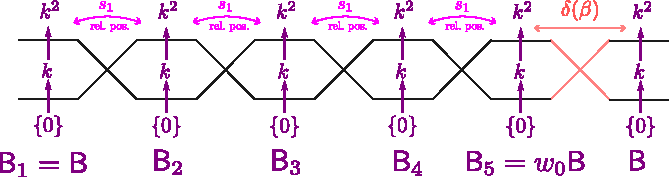
\includegraphics[scale=1]{figures/BraidVariety_Example_2Strands.pdf}
		\caption{The linear configurations of flags parametrized by $X(\s_1^4)$, as in \cref{ex:simple_braidvarieties}.(1). The first flag $\borel_1$ on the left is the standard flag $\{0\}\sse\langle e_1\rangle\sse k^2$, the last flag $\borel_5$ is the antistandard flag $\{0\}\sse\langle e_2\rangle\sse k^2$.}
		\label{fig:BraidVariety_Example_2Strands}
	\end{figure}
\end{center}

\noindent If the reader is not familiar with the types of varieties discussed above, the following explicit examples might be helpful:

\begin{example}\label{ex:simple_braidvarieties}
(1) Consider the braid $\beta=\s_1^n\in\Br(\SL_2)$. The Weyl group $S_2=W(\SL_2)=\langle s_1\rangle$ is generated by a single order-2 transposition, a complete flag in $k^2$ is given by a line $k\sse k^2$, and two lines $\ell_1\stackrel{s_1}{\to}\ell_2$ are in $s_1$-relative position if and only if $\ell_1\neq\ell_2$. The standard flag associated to the upper-triangular Borel $\borel\sse \SL_2$ is given by the line $\langle e_1\rangle\sse k^2$, spanned by $e_1=(1,0)\in k^2$, and the antistandard flag is given by $\langle e_2\rangle\sse k^2$, spanned by $e_2=(0,1)$. The associated braid variety can be described as:
$$X(\s_1^n)\cong\{(\ell_1,\ldots,\ell_{n+1}):\ell_i\subset k^2\mbox{ lines such that }\ell_i\neq\ell_{i+1}, \ell_1=\langle e_1\rangle,\ell_{n+1}=\langle e_2\rangle\}.$$
See Figure \ref{fig:BraidVariety_Example_2Strands} for a visualization. In particular $\dim(X(s_1^n))=n-1$ and it is visibly an affine variety. In simple cases, $X(s_1)=\{\mbox{pt}\}$ is a point and $X(s_1^2)\cong k^\times$, since the space of lines in $k^2$ different from both $\langle(1,0)\rangle$ and $\langle(0,1)\rangle$ is given by the graphs of non-zero linear maps from $k$ to $k$. In general, the varieties $X(\s_1^n)$ are rather interesting for arbitrary $n\in\N$.\\

\noindent (2) Consider the braid $\beta=c^nw_0\in\Br(\SL_{m})$, where $c=\s_1\s_2\cdots \s_{m-1}$ is a Coxeter element, $m\leq n$, and $\ell=\ell(\beta)=n(m-1)+{m\choose 2}$. A point in the braid variety $X(\beta)$ is given by a tuple $(\borel_1,\ldots,\borel_{\ell+1})$ of $(\ell+1)$ full flags in $k^{m}$ satisfying certain conditions. From the piece of $\beta$ corresponding to $c^n$, let $w_1,\ldots,w_n\in k^m$ be vectors such that $\langle w_i\rangle$ coincides with the 1-dimensional subspace of the flag $V_{1+i(m-1)}$, $i\in[1,n]$. Note that in this case the flag $V_{1+j(m-1)}$ is completely determined by $\langle v_j\rangle$ and the flag $V_{1+(j+1)(m-1)}$, $j\in[1,n-1]$, as $V_{1+j(m-1)}$ and $V_{1+(j+1)(m-1)}$ are in $c$-relative position. Using the piece corresponding to $w_0\delta(\b)=w_0^2$, we can construct a set of vectors $w_{n+1},\ldots, w_{m+n}\in k^m$ such that the collection of 1-dimensional vector subspaces $\langle w_i\rangle$ for $i\in[1,n+m]$ uniquely determines a point in $X(\beta)$. Indeed, these vectors $w_j$ are chosen exactly as the previous $w_i$-vectors upon using the identification $c^m=w_0^2$, which holds because $m$ is the Coxeter number. That is, $w_j$ are vectors generating the lines in the corresponding tuples of flags that appears after moving the piece of the braid $w_0^2$ to $c^m$. In terms of such collections of 1-dimensional subspaces, the conditions for the tuple of flags $(\borel_1,\ldots,\borel_{\ell+1})\in X(\beta)$ to belong to the braid variety become
$$w_1\wedge\ldots\wedge w_m\neq 0,\quad w_2\wedge\ldots\wedge w_{m+1}\neq 0,\quad\ldots,\quad w_{n+m}\wedge w_1\wedge\ldots\wedge w_{m-1}\neq 0.$$
Therefore $X(\beta)$ is isomorphic to the locus of the Grassmannian $\Gr(m,n+m)$ where the cyclically consecutive Pl\"ucker coordinates do not vanish quotiented by the corresponding torus.\footnote{The torus quotient is needed, as the dimensions of $X(c^nw_0)$ and $\Gr(m,n+m)$ are $n(m-1)$ and $nm$.} This is known as the top-dimensional open positroid variety, modulo its torus action. Note that the $(-1)$-framed satellite of such $\beta$ along the unknot in $\R^3$ is the $(m,n)$-torus link.\footnote{The 0-framed satellite is the $(m,n+m)$-torus link.} Understood as a max-tb Legendrian link, this explains geometrically the combinatorial relations between invariants of torus links and certain finite point counts on this positroid in $\Gr(m,n+m)$, see e.g.~\cite{LamGalashin_Catalan,GL2023}.\sbs
\end{example}

\begin{comment}
\color{orange}
\noindent It can be enlightening to understand how a braid variety $X(\beta)$ changes when we insert a new crossing to a given braid word $\beta$. The following result, which follows from \cite[Lemma 3.4 \& Section 5.5]{CGGLSS25}, can help build intuition:

\begin{lemma}[Braid varieties under adding crossings]\label{lemma:add_crossing} Let $\beta,\beta'\in\Br_n^+$ be positive braid words such that $\beta'$ is obtained from $\beta$ by inserting one new crossing $\s_i$ somewhere in $\beta$. Then
\begin{enumerate}
\item If $\delta(\beta)=\delta(\b')$, then $X(\beta)\cong X(\beta')$.\\
\item If $\delta(\beta)=\delta(\b')$, then $X(\beta)$ is isomorphic to a codimension-one locally closed subvariety $X(\beta')$.
\end{enumerate}
\end{lemma}
\noindent It might be good to contrast \Cref{lemma:add_crossing} with \Cref{ex:permutation_vs_braid}.
\color{black}
\end{comment}
%%%%%%%%%%%%%%%%%%%%%%%%%%%%%%%%%%%%%%%%%%%%%
%%%%%%%%%%%%%%%%%%%%%%%%%%%%%%%%%%%%%%%%%%%%%
%%%%%%%%%%%%%%%%%%%%%%%%%%%%%%%%%%%%%%%%%%%%%

\subsection{Invariance under braid moves}\label{ssec:braid_varieties_invariance} Let us consider the two braid moves for $\G=\SL_n$:
$$\s_i\s_{i+1}\s_i\to\s_{i+1}\s_i\s_{i+1},\qquad \s_i\s_j\to\s_j\s_i,$$
where $|i-j|\geq2$. In topology, the first move is often referred to as a Reidemeister III (R3) move. The second move can be referred to as a commutation. In terms of the diagrammatics of weaves, these two local braid moves are respectively encoded by the hexavalent and tetravalent vertices, see \Cref{fig:weaves_types_vertices} or \Cref{fig:BraidVariety_DiagramMoves}. Let us now insert flags to these pieces of the weave, building on the diagrammatics from \Cref{sssec:first_connection_weave_diagrams}, see e.g.~\Cref{fig:BraidVariety_DiagramExample}. For that we insert a (horizontal) linear configuration of flags at the horizontal slices above and below the vertex, as in \Cref{fig:BraidVariety_DiagramMoves}. The following result explains how to propagate downwards a tuple of flags in the horizontal slice above a hexavalent or tetravalent vertex:

\begin{center}
	\begin{figure}
		\centering
		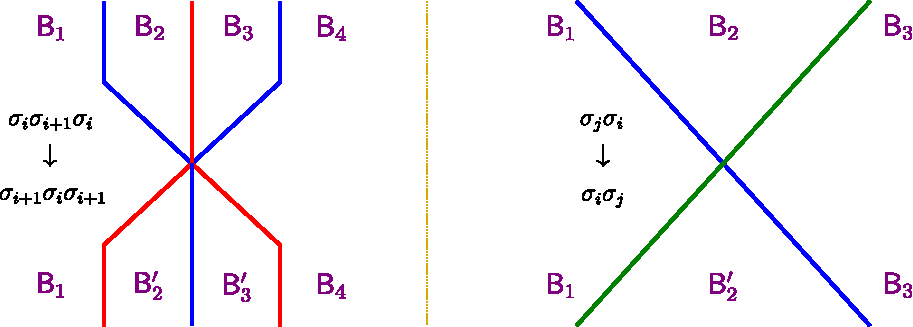
\includegraphics[scale=0.65]{figures/BraidVariety_DiagramMoves.pdf}
		\caption{(Left) A hexavalent weave vertex, with the tuple of flags $(\borel_1,\borel_2,\borel_3,\borel_4)$ along a horizontal slice above the vertex, and tuple of flags $(\borel_1,\borel'_2,\borel'_3,\borel_4)$ below the vertex. \Cref{lem:braid_invariance}.(1) shows that either tuple uniquely determines the other. (Right) A tetravalent weave vertex, with the tuple of flags $(\borel_1,\borel_2,\borel_3)$ above, and $(\borel_1,\borel'_2,\borel_3)$ below the vertex. \Cref{lem:braid_invariance}.(2) shows that either tuple uniquely determines the other.}
		\label{fig:BraidVariety_DiagramMoves}
	\end{figure}
\end{center}

%Braid varieties $X(\beta)$, as in \cref{def:braid_variety}, have a number of interesting symmetries. Some are discussed as follows:
\begin{lemma}[Invariance of $X(\beta)$ under braid moves]\label{lem:braid_invariance}
Let $\beta_1,\beta_2\in\Br(G)$ be two positive $n$-stranded braid words of lengths $\ell_1,\ell_2$. Then:\\

\noindent $(1)$ \underline{R3 move}. For any $i\in[1,n-2]$, consider the regular map
    $$R3_i:X(\beta_1\s_i\s_{i+1}\s_i\beta_2)\lr X(\beta_1\s_{i+1}\s_i\s_{i+1}\beta_2)$$
    \noindent that sends a tuple $(\borel_1,\ldots,\borel_{\ell_1+1},\color{blue}\borel_{\ell_1+2}\color{black},\color{blue}\borel_{\ell_1+3}\color{black},\borel_{\ell_1+4},\ldots,\borel_{\ell_1+\ell_2+4})$ to the tuple
    $$(\borel_1,\ldots,\borel_{\ell_1+1},\color{blue}\borel'_{\ell_1+2}\color{black},\color{blue}\borel'_{\ell_1+3}\color{black},\borel_{\ell_1+4},\ldots,\borel_{\ell_1+\ell_2+4}),$$
    \noindent where the two flags $\color{blue}\borel'_{\ell_1+2}\color{black},\color{blue}\borel'_{\ell_1+3}\color{black}$ are given by

    $$\color{blue}(\borel'_{\ell_1+2})^k\color{black}:=\begin{cases}
			(\borel_{\ell_1+1})^i, & \text{if $k=i$,}\\
            (\borel_{\ell_1+1})^i+(\borel_{\ell_1+4})^i, & \text{if $k=i+1$,}\\
            (\borel_{\ell_1+1})^k, & \text{otherwise,}		 \end{cases}
          \quad \color{blue}(\borel'_{\ell_1+3})^k\color{black}:=\begin{cases}
			(\borel_{\ell_1+4})^i, & \text{if $k=i$,}\\
            (\borel_{\ell_1+1})^i+(\borel_{\ell_1+4})^i, & \text{if $k=i+1$,}\\
            (\borel_{\ell_1+1})^k, & \text{otherwise.}		 \end{cases}$$
    
    \noindent Then $R3_i$ is an isomorphism of algebraic varieties over $\Z$. See Figure \ref{fig:BraidVariety_R3_Invariance} for a visual depiction of the isomorphism $R3_i$.\\

\noindent $(2)$ \underline{Commutation}. For any $i,j\in[1,n-1]$, $2\leq|i-j|$, consider the regular map
    $$C:X(\beta_1\s_i\s_j\beta_2)\lr X(\beta_1\s_j\s_i\beta_2)$$
    \noindent that sends a tuple $(\borel_1,\ldots,\borel_{\ell_1+1},\color{blue}\borel_{\ell_1+2}\color{black},\borel_{\ell_1+3}\color{black},\borel_{\ell_1+4},\ldots,\borel_{\ell_1+\ell_2+3})$ to the tuple
    $$(\borel_1,\ldots,\borel_{\ell_1+1},\color{blue}\borel'_{\ell_1+2}\color{black},\borel_{\ell_1+3}\color{black},\borel_{\ell_1+4},\ldots,\borel_{\ell_1+\ell_2+3}),$$
    where
    $$\color{blue}(\borel'_{\ell_1+2})^k\color{black}:=\begin{cases}
			(\borel_{\ell_1+1})^k, & \text{if $k=i$,}\\
            (\borel_{\ell_1+3})^k, & \text{if $k=j$,}\\
            (\borel_{\ell_1+2})^k, & \text{otherwise.}		 \end{cases}
    $$
    Then $C$ is an isomorphism of algebraic varieties over $\Z$.\\
\end{lemma}

\begin{center}
	\begin{figure}
		\centering
		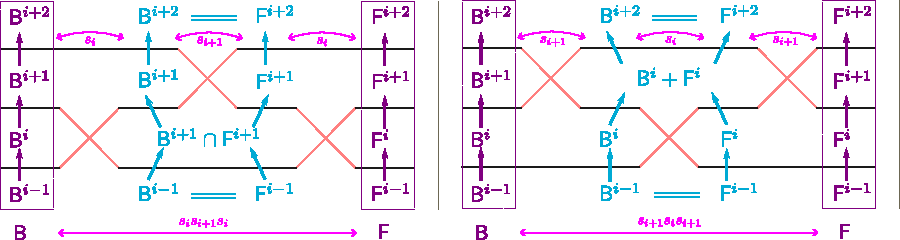
\includegraphics[width=\textwidth]{figures/BraidVariety_R3_Invariance.pdf}
		\caption{The proof of isomorphism invariance of $X(\beta)$ under the Reidemeister 3 ($R3_i$) braid move $\s_i\s_{i+1}\s_i\leftrightarrow\s_{i+1}\s_i\s_{i+1}$, applied to a piece of the braid word $\beta$. (Left) The two flags $\borel,\FF$ at the left and right of $\s_i\s_{i+1}\s_i$, drawn in purple, determine the two intermediate flags in between, drawn in blue. (Right) The two flags $\borel,\FF$ at the left and right of $\s_{i+1}\s_i\s_{i+1}$, in purple, determine the two flags in between, in blue.}
		\label{fig:BraidVariety_R3_Invariance}
	\end{figure}
\end{center}

\begin{comment}
\begin{proof}
For (1), consider the configuration of flags as depicted in Figure \ref{fig:BraidVariety_R3_Invariance}. For a point in $X(\beta_1\s_i\s_{i+1}\s_i\beta_2)$, we have denoted the two flags to the left and right of the piece $\s_i\s_{i+1}\s_i$ by $\borel=\borel_{\ell_1+1}$ and $\FF=\borel_{\ell_1+4}$. The key fact is now that $\borel$ and $\FF$ uniquely determine the two intermediate flags $\borel_{\ell_1+2}$ and $\borel_{\ell_1+3}$; cf.~\cref{ex:permutation_vs_braid}. Indeed, the transversality conditions imply
$$(\borel_{\ell_1+2})^k\color{black}:=\begin{cases}
			\borel^{i+1}\cap\FF^{i+1}, & \text{if $k=i$,}\\
            \borel^k, & \text{otherwise,}		 \end{cases}\quad
    (\borel_{\ell_1+3})^k\color{black}:=\begin{cases}
			\borel^{i+1}\cap\FF^{i+1}, & \text{if $k=i$,}\\
            \FF^k, & \text{otherwise}		 \end{cases}.$$

\noindent After the braid move $\s_i\s_{i+1}\s_i\leftrightarrow\s_{i+1}\s_i\s_{i+1}$, the map $R3_i$ preserves $\borel,\FF$, which are now the flags the same tuple of flags to the left and right of the piece $\s_{i+1}\s_i\s_{i+1}$. Similarly, for this local configuration of four flags at $\s_{i+1}\s_i\s_{i+1}$, the two extreme flags $\borel,\FF$ determine the two intermediate ones $\borel'_{\ell_1+2},\borel'_{\ell_1+3}$ via
$$(\borel'_{\ell_1+2})^k\color{black}:=\begin{cases}
			\borel^{i+1}+\FF^{i+1}, & \text{if $k=i+1$,}\\
            \borel^k, & \text{otherwise,}		 \end{cases}\quad
    (\borel'_{\ell_1+3})^k\color{black}:=\begin{cases}
			\borel^{i+1}+\FF^{i+1}, & \text{if $k=i$,}\\
            \FF^k, & \text{otherwise}		 \end{cases}.$$
\noindent By construction, the map $R3_i$ fixes all the flags in a tuple except for the $(\ell_1+2)$nd and $(\ell_1+3)$rd flags. In particular, $\borel,\FF$ are fixed and by the above they uniquely determine $\borel'_{\ell_1+2},\borel'_{\ell_1+3}$. Thus the map is well-defined and invertible, as required. For (2), just notice that the condition $2\leq|i-j|$ makes the map well-defined and, by construction, it is an isomorphic involution.\end{proof}
\end{comment}
\noindent \cref{lem:braid_invariance} is the reason we use the terminology {\it braid variety} for $X(\beta)$, as it follows that the isomorphism type of $X(\beta)$, as an algebraic variety over $\Z$, only depends on the braid $[\beta]\in\Br(\G)$, rather than the specific choice of word. The proof of \Cref{lem:braid_invariance}.(1) is essentially contained in \Cref{fig:BraidVariety_R3_Invariance}, and Part (2) follows from similar considerations. See \cite[Lemma 3.5]{CGGLSS25} for an alternative proof via coordinates. Another conceptual, more geometric, explanation of the invariance properties in \cref{lem:braid_invariance} is provided by symplectic topology, cf.~\cref{thm:braid_varieties_from_Legendrian}. Note also that \Cref{lem:braid_invariance} applies both ways, since these moves are invertible.\\

From the viewpoint of weaves, \Cref{lem:braid_invariance} has the following consequence. Let $\w$ be a Demazure weave and $v\in\w$ a hexavalent or tetravalent vertex. If $(\borel_1,\ldots,\borel_k)$ is a tuple of flags assigned to a horizontal slice of a Demazure weave $\w$ exactly above $v$, then \Cref{lem:braid_invariance} implies that there exists a unique allowable tuple of flags $(\borel'_1,\ldots,\borel'_k)$ to be assigned to the horizontal slice of $\w$ exactly below $v$. Conversely, a tuple of flags below such a vertex $v$ uniquely determines the tuple above such a vertex $v$. Therefore, we can uniquely propagate a given tuple of flags assigned to a horizontal slice of a Demazure weave up or down past a hexavalent or tetravalent vertex. \Cref{fig:BraidVariety_DiagramMoves} illustrates this propagation locally, with the formulas for $\borel'_2$ and $\borel'_3$ in terms of the flags above given as in \Cref{lem:braid_invariance}.\\

Therefore, at this stage, we can enhance the diagrams for Demazure weaves by inserting compatible tuples of flags at each horizontal slice, and we understand how these propagate past hexavalent and tetravalent vertices. Specifically, if $h_\pm$ are two horizontal slices exactly above and below a hexavalent or tetravalent vertex, as in \Cref{fig:BraidVariety_DiagramMoves2}, and we let $\beta_\pm:=\beta_{h_\pm}$ denote their corresponding braid words, then \Cref{lem:braid_invariance} provides an explicit isomorphism $X(\beta_+)\stackrel{\cong}{\longleftrightarrow}X(\beta_-)$.

\begin{center}
	\begin{figure}
		\centering
		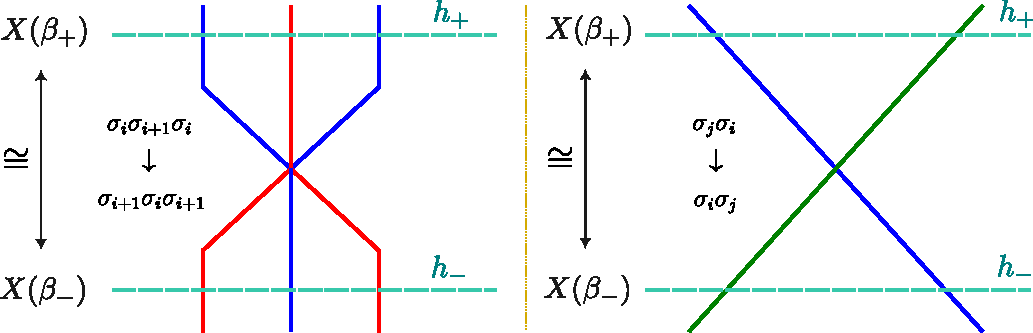
\includegraphics[scale=0.65]{figures/BraidVariety_DiagramMoves2.pdf}
		\caption{(Left) The isomorphism $X(\beta_+)\stackrel{\cong}{\longleftrightarrow}X(\beta_-)$ between the braid varieties given by the horizontal slices above and below a hexavalent vertex is provided in \Cref{lem:braid_invariance}.(1).  (Right) The isomorphism $X(\beta_+)\stackrel{\cong}{\longleftrightarrow}X(\beta_-)$ between the braid varieties given by the horizontal slices above and below a tetravalent vertex is provided in \Cref{lem:braid_invariance}.(2).}
		\label{fig:BraidVariety_DiagramMoves2}
	\end{figure}
\end{center}

A remaining key aspect is to understand what happens to these tuples of flags when we scan downwards past a {\it trivalent vertex}, which we momentarily address in \Cref{ssec:braid_varieties_trivalent}. 

\subsubsection{Further symmetries of braid varieties}\label{sssec:braid_variety_further_symmetries} In addition to \cref{lem:braid_invariance}, there is a cyclic symmetry for braid varieties if $\delta(\beta)=w_0$, which we now assume. Specifically, for any $i\in[1,n-1]$, consider the index $i^*$ such that $s_{i^*}=w_0s_iw_0$, choose $\mathrm{w}\in W(\G)$ with $w_0=\mathrm{w}s_{i}=s_{i^*}\mathrm{w}$ and set $\ell=\ell(\beta)$. Then there exists an isomorphism $R_g^\circlearrowright:X(\s_i\beta)\lr X(\beta \s^*_i)$ of algebraic varieties over $\Z$, see \cite[Section 5.5]{CGGLSS25}. For $\G=\SL_n$, the index is $i^*=n-1$, so that $\s_{i^*}=\s_{n-i}$. Beyond \cref{lem:braid_invariance}, it is also possible to relate certain braid varieties for different ranks $n$ via a Markov-type stabilization process, cf.~\cite[Section 3.2]{CGGS2}. That is, certain braid varieties for $\SL_n$ are isomorphic to those for $\SL_{n+1}$, up to a trivial $\bG_m$-factor. For instance, such isomorphisms capture the $n\leftrightarrow m$ symmetry of $(n,m)$-torus links.\\

Braid varieties have another type of symmetry: they are acted on by a Cartan torus $\T\sse\G$. Since $\T$ fixes the standard and antistandard flags $\borel$ and $w_0\borel$, it follows that the boundary conditions for $X(\beta)$ are preserved, cf.~\cref{eq:braid_variety}. Since $\T$ acts on the flag variety $\G/\borel$ preserving the relative position of pairs of flags, the torus action
\begin{equation}\label{eq:torus_action}
\T\times X(\beta)\lr X(\beta),\quad (\tau;\borel_1,\borel_2,\dots, \borel_{\ell+1})\mapsto (\tau\borel_1,\tau\borel_2,\dots, \tau\borel_{\ell+1})
\end{equation}
is well-defined. In fact, the isomorphisms in \cref{lem:braid_invariance} are $\T$-equivariant, see e.g.~\cite[Section 2.2]{CGGJ24} or \cite[Section 4.5]{CGSS_clusterdeeploci}. The $\T$-action is, in general, not free. For instance, it is not free for $\beta=\s_1^3\in\mbox{Br}_2^+$ as the point $(\borel,\borel_-,\borel,\borel_-)\in X(\s_1^3)$ is fixed. That said, the corresponding $(\T/Z(\G))$-action from \cref{eq:torus_action} is free if $\beta\delta(\beta)$ defines a knot, i.e.~if the decomposition of the permutation $\pi_{\beta\delta(\beta)}\in S_n$ given by the Coxeter projection of $\beta\delta(\beta)$ has a unique factor in its cycle decomposition. In this case, $X(\beta)/(\T/Z(\G))$ is an affine variety and there is an isomorphism $X(\beta)\cong \left(X(\beta)/(\T/Z(\G))\right )\times(\T/Z(\G))$ of algebraic varieties over $\Z$.

\begin{remark}\label{rmk:torus_quasimoment_map} This torus action is part of a quasi-Hamiltonian structure on $X(\beta)$, which further exemplifies the rich geometry of braid varieties. In particular, there is a $\T$-valued moment map $\mu:X(\beta)\lr\T$, where $\T$ acts on the codomain via the $\pi_\beta$-twisted conjugation $(\tau;t)\mapsto (\pi_\beta^{-1}\tau\pi_\b)t\tau^{-1}$.\sbs
\end{remark}
%%%%%%%%%%%%%%%%%%%%%%%%%%%%%%%%%%%%%%%%%%%%%
%%%%%%%%%%%%%%%%%%%%%%%%%%%%%%%%%%%%%%%%%%%%%
%%%%%%%%%%%%%%%%%%%%%%%%%%%%%%%%%%%%%%%%%%%%%

\begin{center}
	\begin{figure}
		\centering
		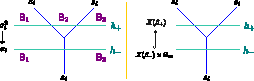
\includegraphics[scale=2.65]{figures/BraidVariety_Trivalent2.pdf}
		\caption{(Left) A trivalent vertex of weave edges labeled by $s_i$, with two horizontal slices $h_\pm$ and the corresponding tuples of flags. In this case, along $h_+$, the relative positions of $(\borel_1,\borel_2,\borel_3)$ are forced to be $\borel_1\stackrel{s_i}{\to}\borel_2$ and $\borel_2\stackrel{s_i}{\to}\borel_3$. Along $h_-$, the relative position of $(\borel_1,\borel_3)$ is $\borel_1\stackrel{s_i}{\to}\borel_3$. (Right) The injective map between the braid varieties, where the braid word $\beta_-$ along $h_-$ is obtained from the word $\beta$ along $h_+$ by applying a $\s_i^2\to\s_i$ move, cf.~\Cref{lem:braidvarieties_trivalent}.}
		\label{fig:BraidVariety_Trivalent2}
	\end{figure}
\end{center}

\subsection{Trivalent weave vertices and braid varieties}\label{ssec:braid_varieties_trivalent} Let us start by studying the local situation of flags near a weave trivalent vertex $v$ for the $\SL_2$-weave $\w:\s_1^2\to\s_1$, as depicted in \Cref{fig:BraidVariety_Trivalent2} (left). At the horizontal slice $h_+$ above $v$ the tuple of flags is of the form $(\borel_1,\borel_2,\borel_3)$, and the relative positions are $\borel_1\stackrel{s_i}{\to}\borel_2$ and $\borel_2\stackrel{s_i}{\to}\borel_3$.\footnote{For now there is merit in not imposing $\borel_1=\borel$ and $\borel_3=s_1\borel$, as maintaining the freedom at the boundary produces a local model that we can insert anywhere in the middle of a braid word to model $\s_i^2\to\s_i$.} At the horizontal slice $h_-$ below $v$ the tuple of flags is of the form $(\borel_1,\borel_3)$, and the relative positions are $\borel_1\stackrel{s_i}{\to}\borel_3$. Therefore, if we are scanning top-to-bottom, implementing the move $\s_i^2\to\s_i$ via a trivalent vertex of a weave, \color{blue}the effect of a trivalent vertex on a tuple of flags as we scan downwards is to impose an additional open condition \color{black} on the tuple of flags above the vertex. In this local model, this is the additional condition $\borel_1\stackrel{s_i}{\to}\borel_3$, which was not necessarily satisfied by all the tuples $(\borel_1,\borel_2,\borel_3)$ along $h_+$.\\

If we read this situation in \Cref{fig:BraidVariety_Trivalent2} (left) from bottom-to-top, the tuple $(\borel_1,\borel_3)$ below determines only two of the flags in the tuple $(\borel_1,\borel_2,\borel_3)$ above. The flag $\borel_2$ can be chosen: since we are in $\SL_2$, and the flag variety is $\SL_2/\borel\cong\PP_k^1$, the choice of $\borel_2$ is given by any point in $(\SL_2/\borel\setminus\{\borel_1,\borel_3\})\cong(\PP_k^1\setminus\{0,\infty\})$. By coordinatizing $(\PP_k^1\setminus\{0,\infty\})$ via $z\in\bG_m$, we conclude that the choices of $\borel_2$ are given by an invertible value $z\in\bG_m$. More generally, by inserting this local model in a positive braid word we obtain the following result:

\begin{lemma}\label{lem:braidvarieties_trivalent}
Let $\beta_1,\beta_2$ be two positive braid words and consider the length $\ell_1:=\ell(\beta_1)-1$. Then there exists a natural open embedding $X(\beta_1\s_i\beta_2)\times\bG_m\hookrightarrow X(\beta_1\s_i^2\beta_2)$ of algebraic varieties over $\Z$ given by
\begin{equation}\label{eq:braidvarieties_trivalent}
(\ldots,\borel_{\ell_1},\borel_{\ell_1+1},\ldots;z)\mapsto (\ldots,\borel_{\ell_1},\color{blue}\borel_{z}\color{black},\borel_{\ell_1+1},\ldots)
\end{equation}
where $\color{blue}\borel_{z}\color{black}$ denotes a flag parametrized by $z\in\bG_m\cong ((\SL_2/\borel)\setminus\{\borel_{\ell_1},\borel_{\ell_1+1}\})$.\sbs
\end{lemma}

\noindent See \Cref{fig:BraidVariety_Trivalent2} (right) for a depiction of \Cref{lem:braidvarieties_trivalent}. The map in \eqref{eq:braidvarieties_trivalent} is typically not surjective. Indeed, any tuple in its image must satisfy $\borel_{\ell_1+1}\stackrel{s_i}{\to}\borel_{\ell_1+2}$, since the domain is $X(\beta_1\s_i\beta_2)$, whereas there is typically no such constraint $\borel_{\ell_1+1}\stackrel{s_i}{\to}\borel_{\ell_1+3}$ in the target $X(\beta_1\s_i^2\beta_2)$.

%%%%%%%%%%%%%%%%%%%%%%%%%%%%%%%%%%%%%%%%%%%%%
%%%%%%%%%%%%%%%%%%%%%%%%%%%%%%%%%%%%%%%%%%%%%
%%%%%%%%%%%%%%%%%%%%%%%%%%%%%%%%%%%%%%%%%%%%%
\subsection{Weave tori in braid varieties}\label{ssec:weave_tori_braid_varieties} Now, given a Demazure weave $\w:\beta\to\delta(\beta)$, we can consider the braid variety $X(\beta)$ as the space of tuples of flags which can be compatibly assigned to the horizontal slice of the north boundary of $\w$. By iteratively scanning top-to-bottom we encounter weave vertices:
\begin{enumerate}
    \item At hexavalent and tetravalent vertices, \Cref{lem:braid_invariance} implies that the tuple of flags can be propagated downwards uniquely {\it without} any loss of information. That is, the braid varieties that arise above and below such vertices are isomorphic, and the particular isomorphism from \Cref{lem:braid_invariance} is chosen to propagate the tuples of flags, cf.~\Cref{fig:BraidVariety_DiagramMoves2}.\\

    \item At a trivalent vertex, \Cref{lem:braidvarieties_trivalent} implies that the tuple of flags can be propagated downwards past the trivalent vertex {\it iff} we impose an additional relative position constraint to the above tuple of flags. \Cref{lem:braidvarieties_trivalent} shows that this determines a locus inside the braid variety above which splits up a $\bG_m$ factor, cf.~\Cref{fig:BraidVariety_Trivalent2} (right).\\
\end{enumerate}

In particular, if we consider two horizontal slices $h,h'$ of the weave $\w$, with $h$ below $h'$ and $q$ trivalent vertices in between, then there exists an open embedding $X(\beta_h)\times(\bG_m)^q\hookrightarrow X(\beta)$, cf.~\cite[Section 5]{CGGJ24}. In particular, if we consider $h$ to be a horizontal slice of the south boundary, so $X(\beta_h)$ is a point and $h'$ a horizontal slice of the north boundary, so $X(\beta_{h'})=X(\beta)$, we obtain an open embedding $\iota_\w:(\bG_m)^d\hookrightarrow X(\beta)$ of an algebraic torus, where $d=\dim(X)$. In conclusion, \Cref{lem:braid_invariance} and \Cref{lem:braidvarieties_trivalent} lead to the following:

\begin{fcor}[Weave tori $T_\w$ in braid varieties]\label{cor:weave_to_toric_embedding}
Let $\beta\in\Br_n^+$ be a positive braid word, $X(\beta)$ its braid variety and $d:=\dim(X)$ its dimension. Consider a Demazure weave $\w:\beta\lr\delta(\beta)$ with $d$ trivalent vertices. Then:
\begin{enumerate}[label=$(\roman*)$]
    \item There exists an open toric embedding
\begin{equation}\label{eq:weave_tori_map}
\iota_\w:(\bG_m)^d\hookrightarrow X(\beta)
\end{equation}
whose image is uniquely determined by assigning flags in $\SL_n/\borel$ to each face of $\w$ such that:\\
\begin{enumerate}[label=$(\alph*)$]
    \item the relative position of such flag is determined by the weave edges, so that two flags $\borel_l,\borel_r$ to the left and right of a weave $s_i$-edge are forced to be in $s_i$-relative position.\\
    \item the leftmost flag must be $\borel$, and the rightmost flag must be $\delta(\beta)\borel$.\\
\end{enumerate}

\item If two Demazure weaves $\w,\w':\beta\lr\delta(\beta)$ are weave equivalent $\w\simeq\w'$, then the images of the corresponding open embeddings $\iota_\w$ and $\iota_{\w'}$ coincide.\\
\item If two Demazure weaves $\w,\w':\beta\lr\delta(\beta)$ are not weave equivalent $\w\not\simeq\w'$, then the images of the corresponding open embeddings $\iota_\w$ and $\iota_{\w'}$ do not coincide.\sbs
\end{enumerate}
\end{fcor}
\vspace{0.2cm}
\noindent \Cref{cor:weave_to_toric_embedding}.$(ii)$ requires a few computations beyond the discussion above, cf.~\cite[Section 5.3]{CGGLSS25}, and \Cref{cor:weave_to_toric_embedding}.$(iii)$ follows from \cite[Theorem 1.1]{CGGLSS25} and \cite[Prop.~ 5.3]{CaoKellerQin22}. We denote the image of $\iota_\w$ in $X(\beta)$ by $T_\w\sse X(\beta)$ and refer to $T_\w$ as a weave torus. A fundamental non-trivial aspect of Demazure weaves is that \color{blue}there are enough Demazure weaves $\w:\beta\to\delta(\beta)$ so that the corresponding collection of weave tori $T_\w$ covers $X(\beta)$ up to codimension two\color{black}. In particular, by the algebraic Hartogs' lemma, the coordinate ring $k[X(\beta)]$ can be entirely studied by using such open tori $T_\w$.\footnote{In fact, $\dim(X)+1$ suffice for such a covering.}

\begin{remark}
More generally, given a weave $\w\sse S$ in a smooth surface $S$, we can consider the flag moduli $\M_\w$ associated to $\w$, as in \cite[Section 5.2]{CasalsZaslow} and see also \cite[Section 5.1]{CGGJ24}. In the case of Demazure weave $\w$, its flag moduli $\M_\w$ is closely related to the weave tori $T_\w$.\sbs
\end{remark}

\subsection{Summary of section}\label{ssec:summary_braid varieties} At this stage we have the following summary of mathematical objects and their relations:
\begin{enumerate}
    \item Given a positive braid word $\beta$, we can consider its braid variety $X(\beta)$, as in \Cref{def:braid_variety}. As illustrated in \Cref{ssec:braid_varieties_examples}, braid varieties generalize a number of important varieties considered in the literature.\\
    
    \item Given a Demazure weave $\w:\beta\to\delta(\b)$, \Cref{cor:weave_to_toric_embedding} provides an open torus $T_\w\sse X(\beta)$. By construction, this open torus $T_\w$ is obtained by imposing further relative position constraints to the tuples of flags giving the points in $X(\beta)$. These additional relative position constraints are dictated by the diagram of $\w$.\\

    \item Given a Demazure weave $\w:\beta\to\delta(\b)$, we can consider the Lusztig cycles $\{\g_v\}$, as in \Cref{def:Lusztig_cycles}, and \Cref{def:intersection_number} provides a quiver $Q_\w$ encoding their intersections.\\
\end{enumerate} 
\Cref{cor:weave_to_toric_embedding} and \Cref{cor:quiver_cycles_weave_operations} imply that both $T_\w$ and $Q_\w$ remain the same under weave equivalences applied to $\w$, and they necessarily change under a weave mutation.\footnote{The resulting quiver $Q_\w$ might, nevertheless, be abstractly isomorphic to $Q_\w$, but $T_\w$ will be genuinely different.}\\

Let $\beta\in\Br_n^+$ be a positive braid word, $\w:\beta\to\delta(\beta)$ a Demazure weave and $X(\beta)$ its braid variety.\\

\noindent Our next task will be to explain how each Lusztig cycle $\g_v$ and each dual Lusztig cycle $\rho_v$ respectively define a rational function $X_{\g_v}\in\Z(X(\beta))$ and a regular function $A_{\r_v}\in\Z[X(\beta)]$. These functions will be the cluster $X$-variables and cluster $A$-variables associated to the quiver $Q_\w$, geometrically realized as elements of the rational field of functions $\Z(X(\beta))$ and the coordinate ring of functions $\Z[X(\beta)]$ of the braid variety $X(\beta)$.

